\section{Completed conditional forecast calibration}

\label{sec:s05-completed}

Each model and California origin has 999 conditional simulated futures and its observed vector. The following tests condition on the fitted state and past history; they do not integrate parameter-estimation uncertainty.

\begin{table}[htbp]\centering\caption{Conditional count, original minimum-rank and continuous-coordinate pooled tests. All p-values use their declared inclusive-tail conventions.}\label{tab:s05-completed}

\begin{tabular}{llrrrr}\toprule Model & Fold & Conditional $N$ & Min-rank & Quadratic & Fisher-type\\\midrule

OC & 0 & 0.002 & 0.070 & 0.004 & 0.001 \\

OC & 1 & 0.594 & 0.075 & 0.003 & 0.004 \\

OC & 2 & 0.056 & 0.069 & 0.007 & 0.012 \\

EP & 0 & 0.002 & 0.070 & 0.004 & 0.002 \\

EP & 1 & 0.698 & 0.075 & 0.005 & 0.006 \\

EP & 2 & 0.036 & 0.069 & 0.009 & 0.008 \\

\bottomrule\end{tabular}\end{table}

The conditional count summary retains lower and upper inclusive empirical tails and reports twice the smaller tail, capped at one. The original minimum-rank test is retained with its exclusions and tie behaviour; it is not replaced by the continuous-coordinate statistics.

The pooled quadratic statistic uses eight declared coordinates: total exposure, time-event log sum, gap KS, gap serial correlation, spatial Rosenblatt KS maximum, absolute spatial cross-correlation, and dimensionless location-log-density mean and variance. Standardization and the ridge-regularized covariance are computed symmetrically on the observed vector plus all simulated vectors. The Fisher-type statistic is the preserved $-\sum_j\log\widetilde p_j$, not an independently calibrated chi-square reference or an assumption of independent coordinates. Both statistics use the inclusive upper rank in the same symmetric pool.

\begin{table}[htbp]\centering\caption{Retained-coordinate and tie diagnostics. Equal counts include the observed vector and every exactly tied pooled statistic.}

\begin{tabular}{llrrr}\toprule Model & Fold & Min-rank coordinates & Quadratic equal & Fisher equal\\\midrule

OC & 0 & 82 & 1 & 1 \\

OC & 1 & 82 & 1 & 1 \\

OC & 2 & 82 & 1 & 1 \\

EP & 0 & 82 & 1 & 1 \\

EP & 1 & 82 & 1 & 1 \\

EP & 2 & 82 & 1 & 1 \\

\bottomrule\end{tabular}\end{table}

Continuous does not automatically mean tie-free: coordinate duplicates and equality with the observed statistic are retained in the public aggregate and interpreted conservatively. This is the declared conditional calibration and pooled omnibus scope. No CSEP L-, M- or S-test results are inferred, and a non-rejection is not proof that the model or physical inhibition mechanism is correct. The independent reconstruction coverage is reported separately below; saved arithmetic checks and raw replay remain distinct forms of evidence.

\begin{figure}[htbp]\centering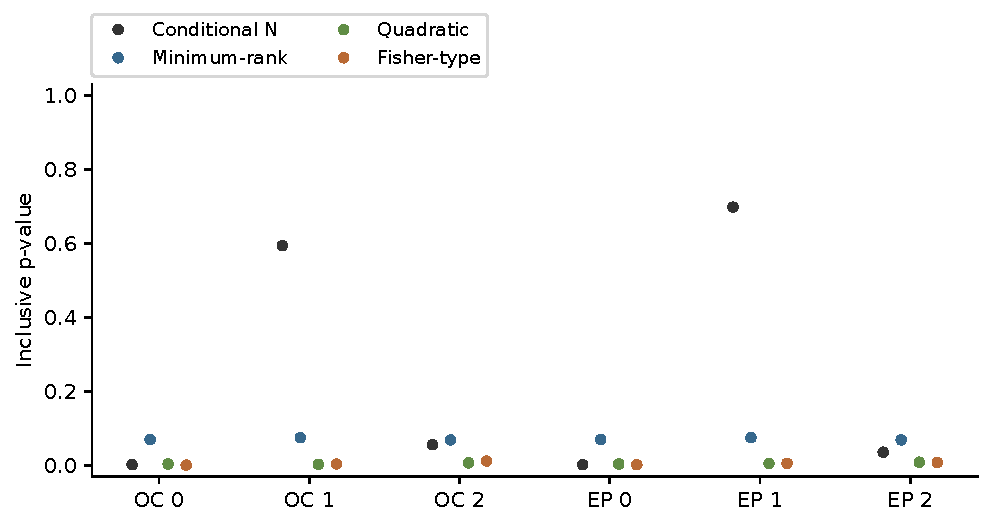
\includegraphics[width=\textwidth]{s05_conditional_pvalues.pdf}\caption{Reported inclusive conditional/pooled p-values.}\end{figure}

\begin{center}\begin{tabular}{llrrl}\toprule Model & Fold & Completed futures & Planned futures & Status\\\midrule

OC & 0 & 999 & 999 & resolved \\

OC & 1 & 999 & 999 & resolved \\

OC & 2 & 999 & 999 & resolved \\

EP & 0 & 999 & 999 & resolved \\

EP & 1 & 999 & 999 & resolved \\

EP & 2 & 999 & 999 & resolved \\

\bottomrule\end{tabular}\end{center}

Both continuous-statistic omnibus procedures reject at the declared five-percent level for each model and origin, while the retained minimum-rank procedure does not. Thus the EP score advantage is not a conditional-adequacy certificate. These are separate within-origin tests, not a joint cross-origin or model-selection-adjusted rejection. The historical OC full-vector audit remains separate.

% Additive replacement audit-scope text for 12_s05_completed.tex.
% Preserve every existing calibration p-value, table and figure.
The original completed independent closure reconstructed count, marks, immigrant and triggering exposure, temporal event logs, and spatial point, location and joint scores directly from all 5,994 saved OC and EP futures (999 per model and origin). It also reconstructed all 84 diagnostic coordinates and all 11 event-detail columns on EP indices 0, 249, 499, 749 and 998 in each of the three origins, giving 15 predeclared full-vector replays. Count identities are exact; finite numerical discrepancies satisfy the declared score, diagnostic and spatial-CDF tolerances. This extends the earlier nine-path native sample and zero-full-vector scope; it does not assert full spatial-PIT replay on all futures.

The independent reconstruction uses incomplete-beta line integrals and a separately implemented positive-polar rectangle-integration kernel. The scoring route and source identities are documented in \path{reproduction/regional/README.md}.

\begin{center}\begin{tabular}{lr}\toprule Independent closure quantity & Value\\\midrule
Independent raw point-score paths & 5994 \\
EP paths with all 84 diagnostics & 15 \\
Maximum point-score error (nats) & 1.17143e-09 \\
Maximum full-vector score error (nats) & 9.09495e-12 \\
Maximum other diagnostic error & 8.18545e-12 \\
Maximum spatial-CDF error & 6.66134e-15 \\
Maximum event-log error (nats) & 1.10134e-13 \\
Maximum gap error & 1.15463e-14 \\
\bottomrule\end{tabular}\end{center}

